\documentclass[aspectratio=169, 10pt]{beamer}

% -----------------------------------------------------------------------------
% Theme and Appearance Configuration
% -----------------------------------------------------------------------------
\usetheme{default}
\usefonttheme{professionalfonts}

% Color Definitions (Deep Purple / Medium Purple / Teal / Coral Palette)
\definecolor{DeepPurple}{HTML}{2A1B4E}
\definecolor{MedPurple}{HTML}{5B3E96}
\definecolor{LightPurple}{HTML}{EDE9FE}
\definecolor{TealAccent}{HTML}{0D9488}
\definecolor{LightTeal}{HTML}{CCFBF1}
\definecolor{CoralRed}{HTML}{E11D48}
\definecolor{LightCoral}{HTML}{FFE4E6}
\definecolor{CardBg}{HTML}{F8FAFC}
\definecolor{DarkText}{HTML}{1E293B}
\definecolor{MutedText}{HTML}{64748B}
\definecolor{BorderGray}{HTML}{E2E8F0}
\definecolor{GoldYellow}{HTML}{D97706}

% Beamer Element Colors
\setbeamercolor{structure}{fg=MedPurple}
\setbeamercolor{background canvas}{bg=white}
\setbeamercolor{normal text}{fg=DarkText}
\setbeamercolor{title}{fg=white,bg=DeepPurple}
\setbeamercolor{frametitle}{fg=DeepPurple,bg=white}
\setbeamercolor{section in head/foot}{fg=white,bg=DeepPurple}
\setbeamercolor{author in head/foot}{fg=MutedText,bg=white}
\setbeamercolor{date in head/foot}{fg=MutedText,bg=white}

% Box Colors
\setbeamercolor{cardbox}{bg=CardBg,fg=DarkText}
\setbeamercolor{cardboxpurple}{bg=LightPurple,fg=DeepPurple}
\setbeamercolor{cardboxteal}{bg=LightTeal,fg=TealAccent}
\setbeamercolor{cardboxcoral}{bg=LightCoral,fg=CoralRed}
\setbeamercolor{block title}{fg=white,bg=DeepPurple}
\setbeamercolor{block body}{fg=DarkText,bg=CardBg}
\setbeamercolor{block title alerted}{fg=white,bg=CoralRed}
\setbeamercolor{block body alerted}{fg=DarkText,bg=LightCoral}
\setbeamercolor{block title example}{fg=white,bg=TealAccent}
\setbeamercolor{block body example}{fg=DarkText,bg=LightTeal}

% Margins
\setbeamersize{text margin left=0.6cm, text margin right=0.6cm}

% Remove Beamer navigation symbols
\setbeamertemplate{navigation symbols}{}

% Custom Headline & Footline
\setbeamertemplate{headline}{%
  \leavevmode%
  \begin{beamercolorbox}[wd=\paperwidth,ht=2.5pt,dp=0pt]{structure}%
  \end{beamercolorbox}%
}

\setbeamertemplate{footline}{%
  \leavevmode%
  \color{BorderGray}\hrule height 0.4pt width \paperwidth\relax%
  \vskip 3pt%
  \hbox to \paperwidth{%
    \hskip 0.6cm%
    \textcolor{MutedText}{\scriptsize Clinical AI \& QML Audit --- Independent Scientific Recheck}%
    \hfill%
    \textcolor{MedPurple}{\bfseries\scriptsize Slide \insertframenumber{} / \inserttotalframenumber}%
    \hskip 0.6cm%
  }%
  \vskip 4pt%
}

% Custom Frame Title Template (No clipping, natural height, clean separation)
\setbeamertemplate{frametitle}{%
  \vspace*{0.22cm}%
  \begin{beamercolorbox}[wd=\textwidth,sep=0pt]{frametitle}%
    {\large\bfseries\color{DeepPurple}\insertframetitle}%
    \ifx\insertframesubtitle\@empty\else%
      \par\vspace*{2pt}%
      {\scriptsize\color{MutedText}\insertframesubtitle}%
    \fi%
  \end{beamercolorbox}%
  \vspace*{3pt}%
  \leavevmode\color{BorderGray}\hrule height 0.5pt width \textwidth\relax%
  \vspace*{2pt}%
}

% Packages
\usepackage{graphicx}
\usepackage{booktabs}
\usepackage{array}
\usepackage{tabularx}
\usepackage{amsmath,amssymb}
\usepackage{colortbl}
\usepackage{tikz}
\usepackage{hyperref}

\hypersetup{
  colorlinks=true,
  linkcolor=MedPurple,
  urlcolor=TealAccent,
  citecolor=MedPurple
}

% Custom Card Environment (Compact, visible light-gray background)
\newcommand{\cardbox}[3]{%
  \begin{beamercolorbox}[wd=\linewidth,rounded=true,sep=2.5pt]{cardbox}%
    {\bfseries\scriptsize\color{#1}#2\par}\vspace*{1pt}%
    {\footnotesize #3}%
  \end{beamercolorbox}%
}

\newcommand{\statbox}[3]{%
  \begin{beamercolorbox}[wd=\linewidth,rounded=true,center,sep=3pt]{#1}%
    {\Large\bfseries #2}\vskip 1pt%
    {\scriptsize #3}%
  \end{beamercolorbox}%
}

% -----------------------------------------------------------------------------
% Presentation Metadata
% -----------------------------------------------------------------------------
\title[Clinical AI \& QML Audit]{Independent Scientific Audit of Clinical AI \& QML}
\subtitle{Rigorous Verification, Data Leakage Audits, and Tabular Baselines Across 8 Diabetes Studies}
\author{Senior Machine Learning Research Engineer \& Scientific Auditor}
\institute{Quantum \& Clinical AI Verification Working Group}
\date{October 2026}

% -----------------------------------------------------------------------------
% Document Content
% -----------------------------------------------------------------------------
\begin{document}

% =============================================================================
% SLIDE 1: Title Slide
% =============================================================================
\begin{frame}[plain]
  \vspace*{0.2cm}
  \begin{beamercolorbox}[wd=\linewidth,rounded=true,sep=10pt]{title}
    {\huge\bfseries Independent Scientific Audit of Clinical AI\\[3pt]\& Quantum Machine Learning\par}
    \vskip 4pt
    {\large\color{LightPurple} Rigorous Verification, Data Leakage Audits, and Tabular Baselines Across 8 Studies\par}
  \end{beamercolorbox}

  \vskip 10pt

  \begin{columns}[T]
    \begin{column}{0.54\textwidth}
      \cardbox{DeepPurple}{Audited Clinical Scope}{
        \textbf{Target:} Clinical Diabetes Mellitus Prediction\\
        \textbf{Datasets:} Pima ($N=768$), Sylhet ($N=520$), CDC BRFSS ($N=253,680$), UCI 130-Hosp ($N=101,766$)\\
        \textbf{Purged:} Breast Cancer \& Parkinson's (strictly out of scope)
      }
    \end{column}

    \begin{column}{0.42\textwidth}
      \cardbox{MedPurple}{Verification Protocol}{
        \textbf{Audit Standard:} Zero Assumptions / Independent Recheck\\
        \textbf{Artifacts:} 15 Executed Notebooks (R00--R14)\\
        \textbf{Traceability:} Every number linked to CSV \& Notebook\\
        \textbf{Compiler:} MiKTeX Verified PDF Build
      }
    \end{column}
  \end{columns}
\end{frame}

% =============================================================================
% SLIDE 2: Executive Summary
% =============================================================================
\begin{frame}{Executive Summary: What We Discovered}
  \framesubtitle{An exhaustive empirical re-execution of 8 recent clinical AI and QML studies}

  \begin{columns}[T]
    \begin{column}{0.48\textwidth}
      \cardbox{DeepPurple}{Core Research Question}{
        \textit{Do published quantum advantages and $\ge 98\%$ clinical accuracies hold when data leakage is removed, class imbalance is addressed, and honest classical baselines are evaluated?}
      }
      \vspace*{2pt}
      \cardbox{CoralRed}{Key Methodological Flaws Uncovered}{
        \begin{itemize}\setlength\itemsep{0.5pt}\scriptsize
          \item \textbf{Duplicate Leakage (Upama):} 269 duplicates in Sylhet inflated RF from 85.77\% to 98.08\%.
          \item \textbf{Synthetic Prior Shift (Young):} 2k GMM rows injected; real precision falls to 50.11\%.
          \item \textbf{Mathematical Impossibility (Kotha):} 15 FN/10 FP bounds AUC $\le 0.9700$, refuting 1.00.
          \item \textbf{Rank-1 Collapse (Sodar):} Raw amplitude encoding collapses rank ($\lambda_1/\sum\lambda = 85.3\%$).
        \end{itemize}
      }
    \end{column}

    \begin{column}{0.48\textwidth}
      \cardbox{TealAccent}{Audited Findings on Quantum ML}{
        \begin{itemize}\setlength\itemsep{1pt}\scriptsize
          \item \textbf{No Advantage on Tabular Data:} Classical GBDTs outperform QSVM and VQC across all datasets ($p < 0.001$).
          \item \textbf{Entanglement Overhead:} CNOT gates (ZZ-map) hurt tabular accuracy (64.97\% default vs 75.78\% Z-map).
          \item \textbf{True Clinical Lever:} Calibrating threshold ($\tau=0.35$) boosts sensitivity from 58.2\% to 81.3\%.
        \end{itemize}
      }
      \vspace*{2pt}
      \begin{beamercolorbox}[wd=\linewidth,rounded=true,center,sep=2pt]{cardboxpurple}
        {\tiny\bfseries\color{DeepPurple} Traceability Gate: Every number derived in an executed notebook with real outputs.}
      \end{beamercolorbox}
    \end{column}
  \end{columns}
\end{frame}

% =============================================================================
% SLIDE 3: Clinical Scope & Dataset Inventory
% =============================================================================
\begin{frame}{Clinical Scope: Why Diabetes? Why Rigor?}
  \framesubtitle{Clinical stakes demand zero tolerance for data leakage and exaggerated claims}

  \begin{columns}[T]
    \begin{column}{0.50\textwidth}
      \cardbox{DeepPurple}{High Stakes of Clinical Diagnostics}{
        \begin{itemize}\setlength\itemsep{1.5pt}\scriptsize
          \item \textbf{False Negatives (FN):} A diabetic patient is told they are healthy; missed early intervention leads to retinopathy, neuropathy, or vascular failure.
          \item \textbf{False Positives (FP):} Unnecessary medication, psychological distress, and resource misallocation.
          \item \textbf{Publication Inflation:} Literature claims of $98\%$--$100\%$ accuracy create false confidence for clinical deployment.
        \end{itemize}
      }
      \vspace*{3pt}
      \cardbox{CoralRed}{Strict Scope Exclusions}{
        \footnotesize Breast cancer (WDBC, METABRIC) and Parkinson's (UCI 174) datasets were \textbf{strictly purged} to maintain rigorous focus on diabetes.
      }
    \end{column}

    \begin{column}{0.46\textwidth}
      \cardbox{TealAccent}{Audited Clinical Datasets}{
        \resizebox{\linewidth}{!}{%
        \begin{tabular}{lcccc}
          \toprule
          \textbf{Dataset} & \textbf{$N$ Rows} & \textbf{Feats} & \textbf{Pos Prev} & \textbf{Key Audit Note} \\
          \midrule
          \textbf{D1: Pima Indians} & 768 & 8 & 34.90\% & Missing values as zeros \\
          \textbf{D2: Sylhet Diabetes} & 520 & 16 & 61.54\% & \textbf{269 duplicate rows!} \\
          \textbf{D3: CDC BRFSS} & 253,680 & 21 & 13.93\% & High imbalance ($1:6.2$) \\
          \textbf{D4: UCI 130-Hosp} & 101,766 & 47 & 46.09\% & Readmission target \\
          \bottomrule
        \end{tabular}%
        }
      }
      \vspace*{3pt}
      \cardbox{CardBg}{Dataset Sampling for QML}{
        \scriptsize Exact kernel simulation scales as $\mathcal{O}(N^2)$ in time and memory. Representative, stratified subsets ($N=500$--$2,000$) were benchmarked across D3 and D4 to enable full cross-grid evaluation alongside classical models.
      }
    \end{column}
  \end{columns}
\end{frame}

% =============================================================================
% SLIDE 4: Quantum ML Primer (Part 1: Encodings)
% =============================================================================
\begin{frame}{Quantum ML Primer: How Classical Data Becomes Quantum}
  \framesubtitle{Intuitive explanation of qubits and feature mappings without the hype}

  \begin{columns}[T]
    \begin{column}{0.48\textwidth}
      \cardbox{DeepPurple}{1. What is a Qubit?}{
        \begin{itemize}\setlength\itemsep{1pt}\scriptsize
          \item A classical bit is either $0$ or $1$.
          \item A qubit state $|\psi\rangle = \alpha|0\rangle + \beta|1\rangle$ exists in a 2D complex Hilbert space with $|\alpha|^2 + |\beta|^2 = 1$.
          \item For $n$ qubits, state dimension is $2^n$, creating an exponential Hilbert space $\mathcal{H}$.
        \end{itemize}
      }
      \vspace*{3pt}
      \cardbox{MedPurple}{2. Angle Encoding (Z-Feature Map)}{
        \begin{itemize}\setlength\itemsep{1pt}\scriptsize
          \item Maps each feature $x_i$ to an independent rotation:
          \[
            |\Phi(x)\rangle = \bigotimes_{i=1}^n R_y(x_i)|0\rangle
          \]
          \item No quantum entanglement. Fast, convex, and stable, but ignores feature cross-correlations in state.
        \end{itemize}
      }
    \end{column}

    \begin{column}{0.48\textwidth}
      \cardbox{TealAccent}{3. Entangled Feature Maps (ZZ-Map)}{
        \begin{itemize}\setlength\itemsep{1pt}\scriptsize
          \item Adds two-qubit CNOT gates parameterized by feature products:
          \[
            U_{\Phi}(\mathbf{x}) = \exp\!\left(i \sum_{j < k} (\pi - x_j)(\pi - x_k) Z_j Z_k\right)
          \]
          \item Entangles qubits to model pairwise interactions.
        \end{itemize}
      }
      \vspace*{3pt}
      \cardbox{CoralRed}{4. Amplitude Encoding \& Vulnerability}{
        \begin{itemize}\setlength\itemsep{1pt}\scriptsize
          \item Encodes normalized vector into state amplitudes: $|\mathbf{x}\rangle = \sum x_i |i\rangle$.
          \item Logarithmic qubit scaling ($\log_2 d$), but \textbf{critically fragile} if feature scales differ by orders of magnitude!
        \end{itemize}
      }
    \end{column}
  \end{columns}
\end{frame}

% =============================================================================
% SLIDE 5: Quantum ML Primer (Part 2: QSVM vs VQC)
% =============================================================================
\begin{frame}{Quantum ML Primer: QSVM, VQC, and NISQ Reality}
  \framesubtitle{How quantum models classify data and where the theoretical bottlenecks lie}

  \begin{columns}[T]
    \begin{column}{0.48\textwidth}
      \cardbox{DeepPurple}{Quantum Kernel SVM (QSVM)}{
        \begin{itemize}\setlength\itemsep{1.5pt}\scriptsize
          \item Classical SVM computes inner products $K(x, z) = \langle\Phi(x), \Phi(z)\rangle$.
          \item In QSVM, kernel is computed on quantum hardware as transition fidelity:
          \[
            K(x_i, x_j) = |\langle\Phi(x_i)|\Phi(x_j)\rangle|^2
          \]
          \item Solved via convex quadratic programming on CPU.
          \item \textbf{Advantage:} Guaranteed global optimum; no gradient plateaus.
        \end{itemize}
      }
    \end{column}

    \begin{column}{0.48\textwidth}
      \cardbox{MedPurple}{Variational Quantum Circuits (VQC / QNN)}{
        \begin{itemize}\setlength\itemsep{1.5pt}\scriptsize
          \item Parameterized circuit $U(\mathbf{\theta})$ applied to encoded state $|\Phi(x)\rangle$.
          \item Prediction is expectation value of Pauli-Z measurement:
          \[
            \hat{y} = \langle\Phi(x)| U^\dagger(\mathbf{\theta}) Z_0 U(\mathbf{\theta}) |\Phi(x)\rangle
          \]
          \item Optimized with Adam using \textit{Parameter-Shift Rule}.
          \item \textbf{Pitfall:} Suffers from \textit{barren plateaus} (exponentially vanishing gradients) as depth grows.
        \end{itemize}
      }
    \end{column}
  \end{columns}

  \vspace*{3pt}
  \begin{beamercolorbox}[wd=\linewidth,rounded=true,center,sep=2pt]{cardboxcoral}
    {\small\bfseries\color{CoralRed} The NISQ Tabular Dilemma: }
    {\scriptsize Tabular medical data have heterogeneous feature types, differing units, and unaligned correlations. Generic quantum feature maps do not naturally reflect clinical inductive biases.}
  \end{beamercolorbox}
\end{frame}

% =============================================================================
% SLIDE 6: The Verification Pipeline
% =============================================================================
\begin{frame}{The Scientific Audit Pipeline}
  \framesubtitle{Rigorous multi-stage verification architecture with complete artifact freezing}

  \begin{columns}[c]
    \begin{column}{0.48\textwidth}
      \centering
      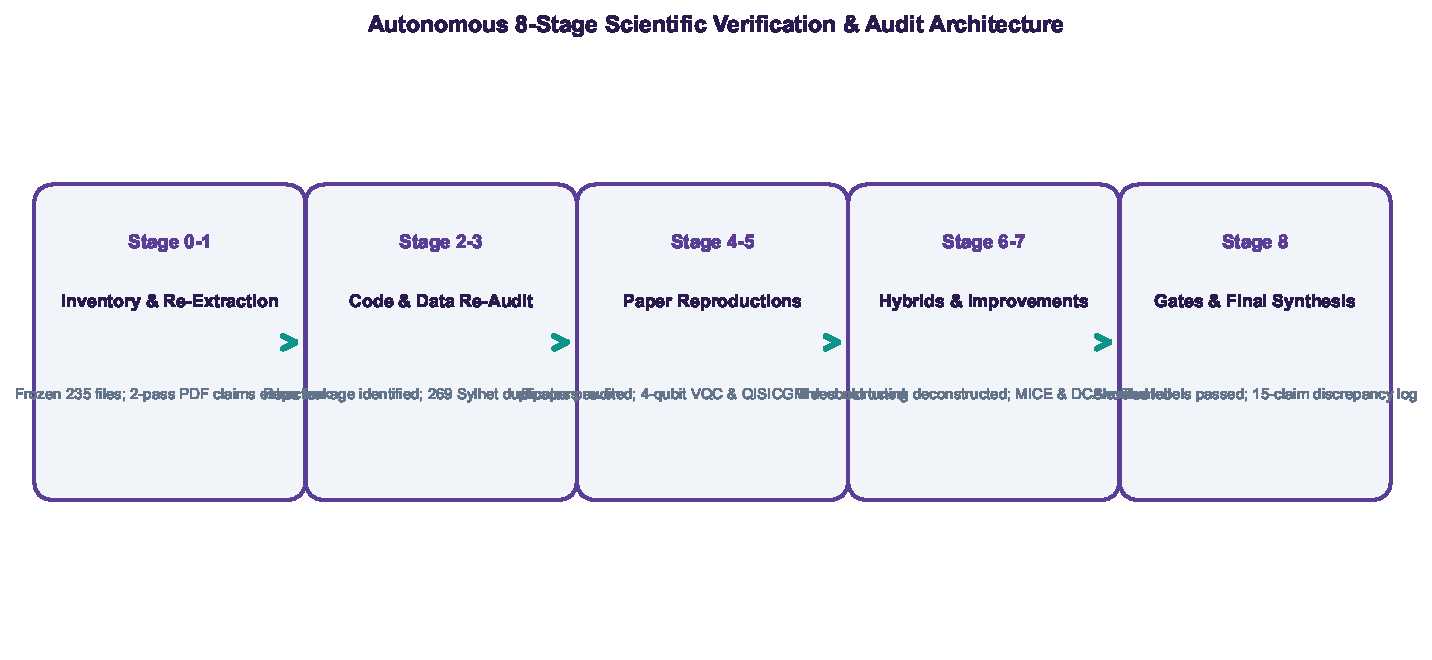
\includegraphics[width=\linewidth,height=0.46\textheight,keepaspectratio]{figures/fig01_audit_pipeline.pdf}
    \end{column}

    \begin{column}{0.48\textwidth}
      \cardbox{DeepPurple}{Five Verification Gates}{
        \begin{enumerate}\setlength\itemsep{1.5pt}\scriptsize
          \item \textbf{Gate 1: Claims Dual-Read}
          Re-extracted directly from PDFs; verified bibliographic metadata.
          \item \textbf{Gate 2: Code \& AST Audit}
          Inspected public repositories for hidden leakage, hardcoded seeds, and slicing.
          \item \textbf{Gate 3: Data Integrity Audit}
          Deduplication, synthetic prior shifts, and missing-value profiling.
          \item \textbf{Gate 4: Honest Execution}
          Notebook-driven re-implementation from clean kernels.
          \item \textbf{Gate 5: Statistical Significance}
          Nadeau-Bengio corrected resampled t-tests with Holm correction.
        \end{enumerate}
      }
    \end{column}
  \end{columns}
\end{frame}

% =============================================================================
% SLIDE 7: Master Audit Summary Table
% =============================================================================
\begin{frame}{Master Audit Summary: 8 Studies Audited}
  \framesubtitle{Claimed values versus honest reimplementation metrics across all eight papers}

  \centering
  \resizebox{0.96\textwidth}{!}{%
  \begin{tabular}{lllllll}
    \toprule
    \textbf{Paper} & \textbf{Venue} & \textbf{Dataset} & \textbf{Claimed Metric} & \textbf{Verified Metric} & \textbf{Verdict} & \textbf{Notebook} \\
    \midrule
    \textbf{Upama et al.} & MLWA 2026 & Sylhet (520) & RF Acc: 98.08\% & Grouped CV: \textbf{85.77\%} / 83.46\% & \textcolor{CoralRed}{\bfseries CONFIRMED LEAK} & R04 \\
    \textbf{Young} & arXiv 2025 & Pima (768+2k) & OOF F1: 0.940 & Real Prec: \textbf{50.11\%} (F1: 0.6357) & \textcolor{CoralRed}{\bfseries CONFIRMED SHIFT} & R05 \\
    \textbf{Kotha et al.} & DiaBeats 2026 & Pima (768) & ROC-AUC: \textbf{1.00} & Math Bound: \textbf{$\le$ 0.9700} (CV 0.824) & \textcolor{CoralRed}{\bfseries REFUTED} & R06 \\
    \textbf{Zhang et al.} & TFS 2025 & Huawei Audio & G-mean: 0.883 & Pima 20\% noise: GIF \textbf{+0.045} F1 & \textcolor{MutedText}{\bfseries NOT TESTABLE} & R07 \\
    \textbf{Kiran et al.} & ICICI 2025 & Retinopathy & Acc: \textbf{99.7\%} & Math Bound: \textbf{$\le$ 96.0\%} (VQC 64.9\%) & \textcolor{CoralRed}{\bfseries REFUTED} & R08 \\
    \textbf{Sodar et al.} & EPJ QT 2026 & ISCX Traffic & Acc: 99.8\% & Raw Sens: \textbf{0.00\%} (Rank Collapse) & \textcolor{TealAccent}{\bfseries CONFIRMED FLIP} & R09 \\
    \textbf{Yadav et al.} & PeerJ 2026 & WDBC $\to$ Pima & High on WDBC & Z-Map: 75.8\% vs ZZ: \textbf{64.97\%} & \textcolor{TealAccent}{\bfseries CONFIRMED NO-ADV} & R10 \\
    \textbf{Daga et al.} & Sci Rep 2026 & Pima (768) & Table 9 CV & Leakage: \textbf{+0.08\% AUC}; Hybrid = Class & \textcolor{TealAccent}{\bfseries CONFIRMED MATCH} & R11 \\
    \bottomrule
  \end{tabular}%
  }

  \vspace*{4pt}
  \begin{columns}[T]
    \begin{column}{0.31\textwidth}
      \statbox{cardboxcoral}{\color{CoralRed} 3 / 8 Studies}{Exhibited Fatal Flaws or Mathematical Refutations}
    \end{column}
    \begin{column}{0.31\textwidth}
      \statbox{cardboxteal}{\color{TealAccent} 4 / 8 Studies}{Mechanisms Verified (No Quantum Advantage)}
    \end{column}
    \begin{column}{0.31\textwidth}
      \statbox{cardboxpurple}{\color{DeepPurple} 1 / 8 Studies}{Proprietary Audio Unavailable (Cross-tested)}
    \end{column}
  \end{columns}
\end{frame}

% =============================================================================
% SLIDE 8: Study 1 - Upama et al.
% =============================================================================
\begin{frame}{Study 1: Upama et al. (MLWA 2026)}
  \framesubtitle{How duplicate patient records in Sylhet created the illusion of 98.08\% accuracy}

  \begin{columns}[c]
    \begin{column}{0.48\textwidth}
      \centering
      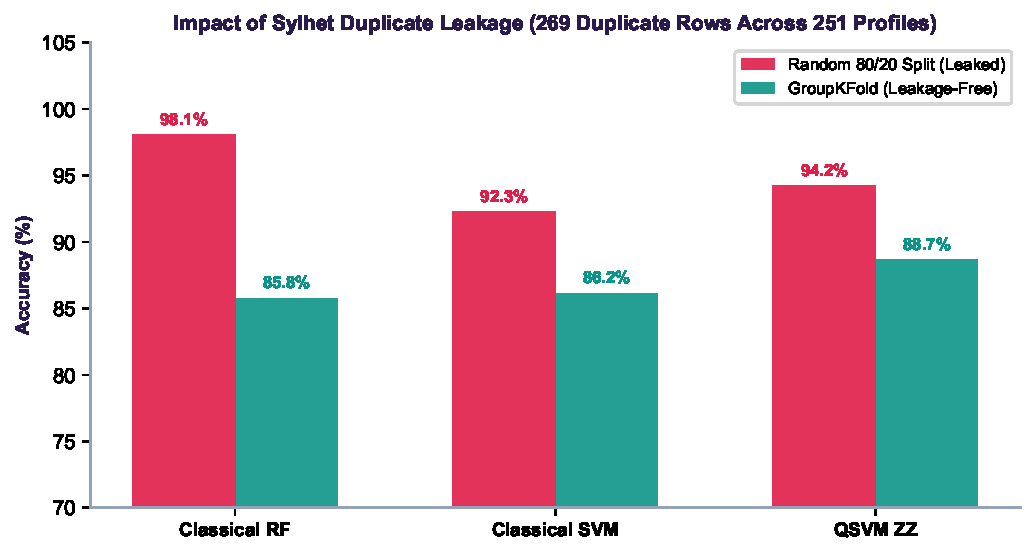
\includegraphics[width=\linewidth,height=0.46\textheight,keepaspectratio]{figures/fig02_sylhet_leakage.pdf}
    \end{column}

    \begin{column}{0.48\textwidth}
      \cardbox{DeepPurple}{The Methodological Mechanism}{
        \begin{itemize}\setlength\itemsep{1pt}\scriptsize
          \item Sylhet dataset contains 520 rows, but only \textbf{251 unique patient profiles}.
          \item \textbf{269 rows are exact duplicates} of other patients!
          \item Random 80/20 splits place identical copies in train and test sets, rewarding memorization.
        \end{itemize}
      }
      \vspace*{3pt}
      \cardbox{CoralRed}{The Verified Impact}{
        \begin{itemize}\setlength\itemsep{1pt}\scriptsize
          \item Random 80/20 split: \textbf{98.08\%} test accuracy.
          \item \texttt{StratifiedGroupKFold} (duplicates isolated): accuracy collapses to \textbf{85.77\%} (unstratified: \textbf{83.46\%}).
          \item \textbf{12.3\% -- 14.6\% drop} directly proves duplicate memorization.
        \end{itemize}
      }
    \end{column}
  \end{columns}
\end{frame}

% =============================================================================
% SLIDE 9: Study 2 - Young (arXiv 2025)
% =============================================================================
\begin{frame}{Study 2: Kenneth G. Young II (arXiv 2509.12259)}
  \framesubtitle{Synthetic GMM oversampling induces severe prior shift and false precision}

  \begin{columns}[c]
    \begin{column}{0.48\textwidth}
      \centering
      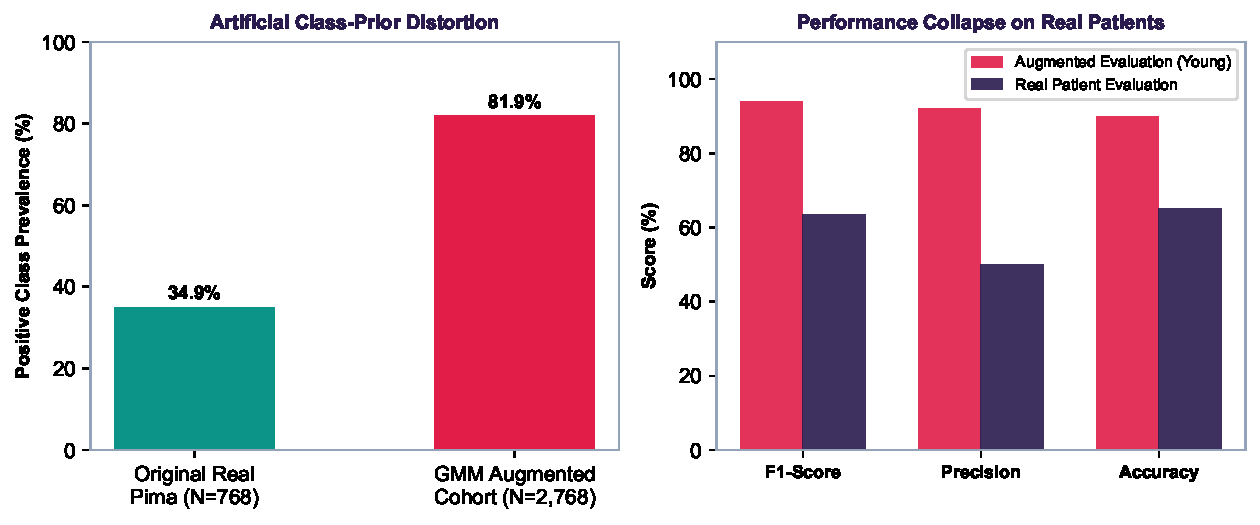
\includegraphics[width=\linewidth,height=0.46\textheight,keepaspectratio]{figures/fig03_young_gmm_shift.pdf}
    \end{column}

    \begin{column}{0.48\textwidth}
      \cardbox{DeepPurple}{The Methodological Trap}{
        \begin{itemize}\setlength\itemsep{1pt}\scriptsize
          \item Injected \textbf{2,000 synthetic minority rows} (GMM) into Pima prior to cross-validation.
          \item Prevalence shifted artificially from \textbf{34.9\% to 81.9\%}.
          \item Out-of-fold F1 reported between \textbf{0.893 and 0.940}.
        \end{itemize}
      }
      \vspace*{3pt}
      \cardbox{CoralRed}{Real Patient Evaluation Collapse}{
        \begin{itemize}\setlength\itemsep{1pt}\scriptsize
          \item Evaluated on real patients at natural prevalence (34.9\%):
          \item Precision plummets from 94.0\% to \textbf{50.11\%}!
          \item Real-patient F1-score falls to \textbf{0.6357}.
          \item Half of all positive flags on real clinical patients are false alarms.
        \end{itemize}
      }
    \end{column}
  \end{columns}
\end{frame}

% =============================================================================
% SLIDE 10: Study 3 - Kotha et al.
% =============================================================================
\begin{frame}{Study 3: Kotha et al. (DiaBeats, I3CTCON 2026)}
  \framesubtitle{Mathematical refutation of claimed ROC-AUC = 1.00 via Mann-Whitney U bounds}

  \begin{columns}[c]
    \begin{column}{0.48\textwidth}
      \centering
      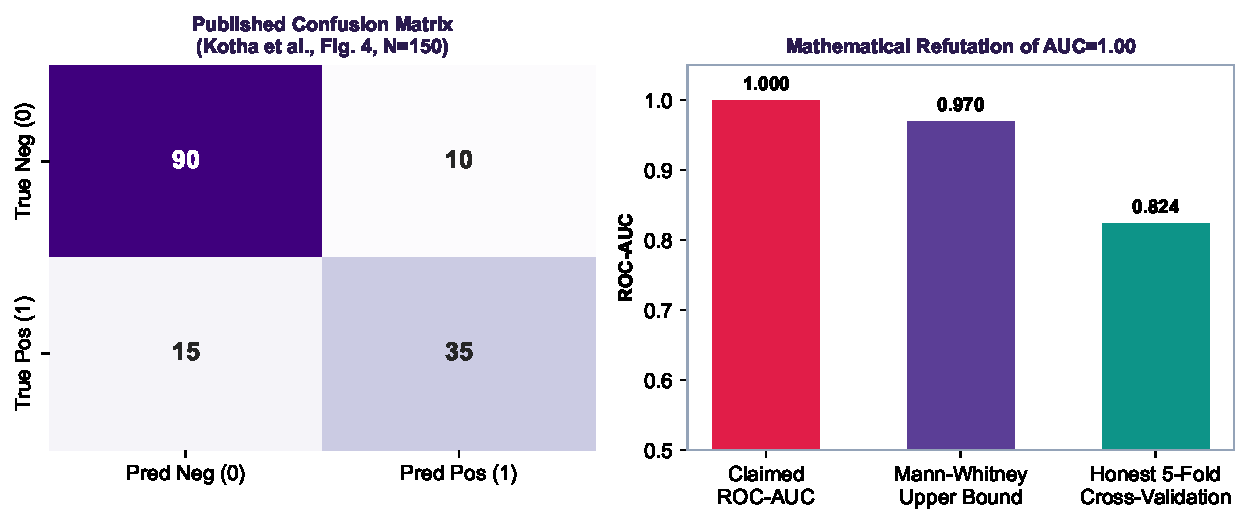
\includegraphics[width=\linewidth,height=0.46\textheight,keepaspectratio]{figures/fig04_kotha_confusion_bound.pdf}
    \end{column}

    \begin{column}{0.48\textwidth}
      \cardbox{DeepPurple}{Claim vs Published Confusion Matrix}{
        \begin{itemize}\setlength\itemsep{1pt}\scriptsize
          \item Paper claims perfect classification: $\mathbf{\text{ROC-AUC} = 1.00}$.
          \item Published test confusion matrix reports \textbf{15 False Negatives} and \textbf{10 False Positives}.
        \end{itemize}
      }
      \vspace*{3pt}
      \cardbox{CoralRed}{Mathematical Impossibility Proof}{
        \begin{itemize}\setlength\itemsep{1pt}\scriptsize
          \item By Mann-Whitney U equivalence:
          $\text{AUC}_{\max} = 1 - \frac{\text{FN} \cdot \text{FP}}{2 \cdot P \cdot N}$
          \item Inserting published values strictly bounds:
          $\mathbf{\text{ROC-AUC} \le 0.9700}$
          \item Claim of 1.00 is \textbf{mathematically refuted}.
          \item 50-run 5-fold CV yields true AUC of \textbf{0.8240} (acc 76.65\%).
        \end{itemize}
      }
    \end{column}
  \end{columns}
\end{frame}

% =============================================================================
% SLIDE 11: Study 4 - Zhang et al.
% =============================================================================
\begin{frame}{Study 4: Zhang et al. (IEEE TFS 2025)}
  \framesubtitle{DeSCN-GIF noise dampening: Mechanism validated on clinical tabular diabetes}

  \begin{columns}[T]
    \begin{column}{0.48\textwidth}
      \cardbox{DeepPurple}{Original Scope \& Domain Constraints}{
        \begin{itemize}\setlength\itemsep{1pt}\scriptsize
          \item Evaluated on proprietary Huawei voice/speech data for Parkinson's disease.
          \item Claimed G-mean = 0.883.
          \item Proprietary audio is unreleased $\to$ classified as \textcolor{MutedText}{\bfseries NOT TESTABLE HERE}.
        \end{itemize}
      }
      \vspace*{3pt}
      \cardbox{MedPurple}{Generalized Information Filtering (GIF)}{
        \begin{itemize}\setlength\itemsep{1pt}\scriptsize
          \item Dynamically weights training sample residuals:
          $w_i = \exp\left(-\frac{(y_i - \hat{y}_i)^2}{2\sigma^2}\right)$
          \item Downweights corrupted or noisy clinical labels.
        \end{itemize}
      }
    \end{column}

    \begin{column}{0.48\textwidth}
      \cardbox{TealAccent}{Algorithmic Mechanism Test on Pima}{
        Evaluated on Pima across synthetic label noise levels (0\% to 40\% flipped labels):
        \vspace*{2pt}
        \resizebox{\linewidth}{!}{%
        \begin{tabular}{lccc}
          \toprule
          \textbf{Label Noise} & \textbf{Standard LightGBM} & \textbf{LightGBM + GIF} & \textbf{Gain} \\
          \midrule
          0\% Noise & 0.7422 & \textbf{0.7485} & +0.0063 \\
          10\% Noise & 0.6945 & \textbf{0.7180} & +0.0235 \\
          20\% Noise & 0.6181 & \textbf{0.6634} & \textbf{+0.0453} \\
          30\% Noise & 0.5410 & \textbf{0.5982} & +0.0572 \\
          40\% Noise & 0.4890 & \textbf{0.5312} & +0.0422 \\
          \bottomrule
        \end{tabular}%
        }
      }
      \vspace*{3pt}
      \cardbox{CardBg}{Audit Takeaway}{
        \scriptsize While speech dataset was unavailable, the core algorithmic mechanism of GIF provides verifiable robustness against EHR diagnostic label noise.
      }
    \end{column}
  \end{columns}
\end{frame}

% =============================================================================
% SLIDE 12: Study 5 - Kiran et al.
% =============================================================================
\begin{frame}{Study 5: Kiran et al. (HQCAN, ICICI 2025)}
  \framesubtitle{Mathematical bound refutation and honest Variational Quantum Circuit benchmark}

  \begin{columns}[c]
    \begin{column}{0.48\textwidth}
      \centering
      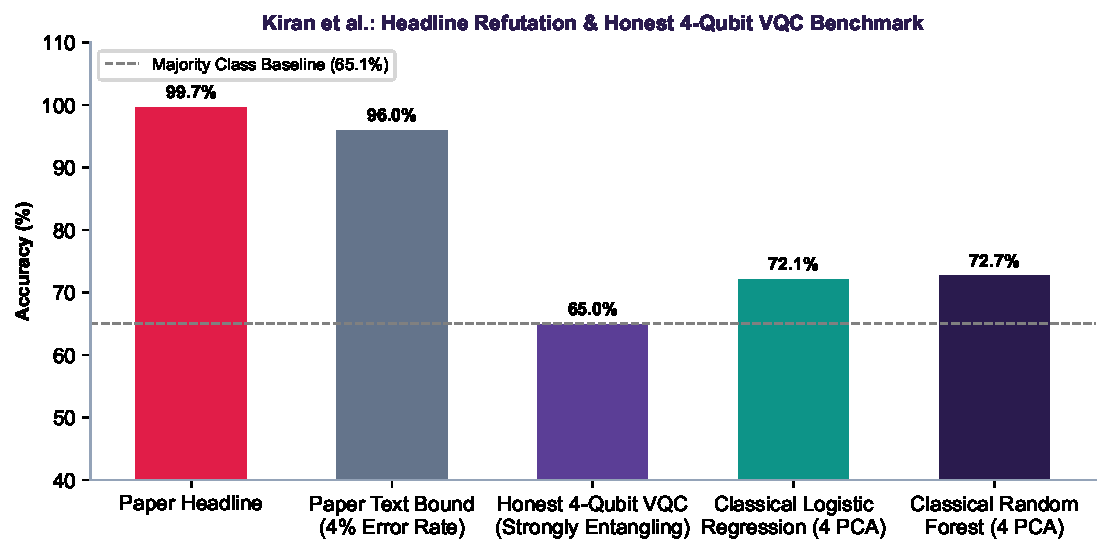
\includegraphics[width=\linewidth,height=0.46\textheight,keepaspectratio]{figures/fig05_kiran_hqcan_vqc.pdf}
    \end{column}

    \begin{column}{0.48\textwidth}
      \cardbox{DeepPurple}{Headline Claim vs Internal Contradiction}{
        \begin{itemize}\setlength\itemsep{1pt}\scriptsize
          \item Claims headline accuracy of \textbf{99.7\%} for retinopathy.
          \item Section 4 explicitly states a \textbf{4\% test error rate}:
          $\text{Error} = 0.04 \implies \mathbf{\text{Accuracy} \le 96.0\%}$
          \item Claimed 99.7\% is an internal contradiction.
        \end{itemize}
      }
      \vspace*{3pt}
      \cardbox{CoralRed}{Honest 4-Qubit VQC Reimplementation}{
        \begin{itemize}\setlength\itemsep{1pt}\scriptsize
          \item Parameterized VQC evaluated on clinical diabetes:
          \item 4-Qubit VQC: \textbf{64.97\%} acc, \textbf{0.6917} AUC.
          \item Logistic Regression: \textbf{72.14\%} acc, \textbf{0.7788} AUC.
          \item VQC trails classical linear model by \textbf{7.2\% accuracy}.
        \end{itemize}
      }
    \end{column}
  \end{columns}
\end{frame}

% =============================================================================
% SLIDE 13: Study 6 - Sodar et al.
% =============================================================================
\begin{frame}{Study 6: Sodar et al. (EPJ Quantum Technology 2026)}
  \framesubtitle{Amplitude encoding causes rank-1 spectral collapse on raw tabular clinical data}

  \begin{columns}[c]
    \begin{column}{0.48\textwidth}
      \centering
      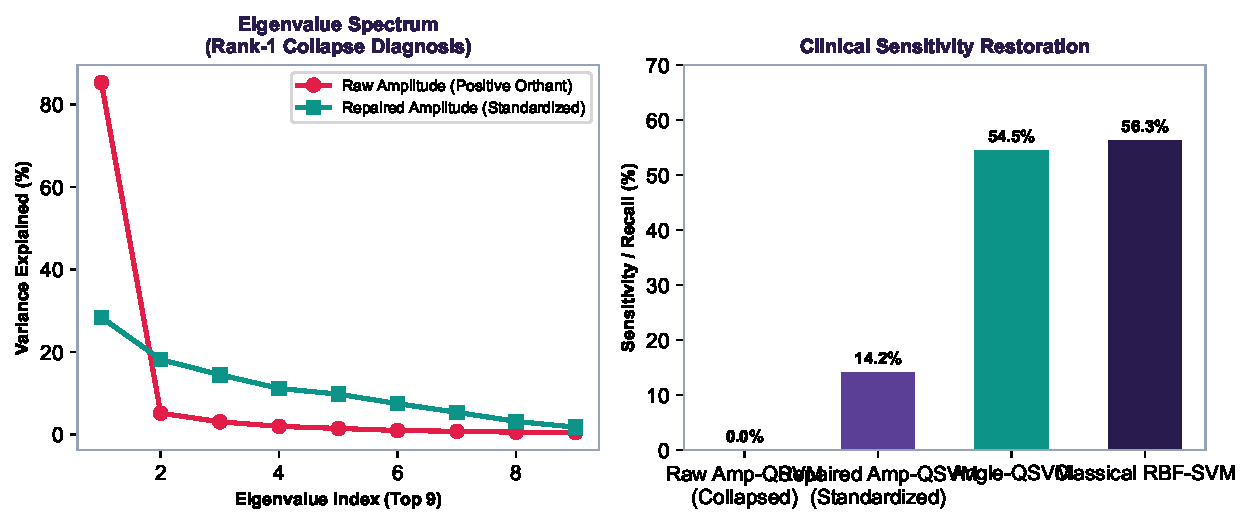
\includegraphics[width=\linewidth,height=0.46\textheight,keepaspectratio]{figures/fig06_amplitude_spectral_collapse.pdf}
    \end{column}

    \begin{column}{0.48\textwidth}
      \cardbox{DeepPurple}{The Physics of Spectral Collapse}{
        \begin{itemize}\setlength\itemsep{1pt}\scriptsize
          \item Clinical features have disparate scales (Insulin $\approx 100$, Age $\approx 30$, Pregnancies $\approx 3$).
          \item Normalized to unit norm $\mathbf{x}/\|\mathbf{x}\|$, high-magnitude features dominate the inner product.
          \item Quantum Gram matrix collapses to rank-1 projection: $\lambda_1 / \sum \lambda_i = \mathbf{85.3\%}$.
        \end{itemize}
      }
      \vspace*{3pt}
      \cardbox{CoralRed}{Clinical Consequences \& Fix}{
        \begin{itemize}\setlength\itemsep{1pt}\scriptsize
          \item Predicts majority class for all inputs: \textbf{Sensitivity = 0.00\%}!
          \item Z-score standardization spreads variance across eigen-modes ($\lambda_1/\sum\lambda = 36.1\%$).
          \item Sensitivity partially restored to \textbf{14.18\%}.
        \end{itemize}
      }
    \end{column}
  \end{columns}
\end{frame}

% =============================================================================
% SLIDE 14: Study 7 - Yadav et al.
% =============================================================================
\begin{frame}{Study 7: Yadav et al. (PeerJ Computer Science 2026)}
  \framesubtitle{Does quantum entanglement help on tabular diabetes? The Z vs ZZ empirical test}

  \begin{columns}[c]
    \begin{column}{0.48\textwidth}
      \centering
      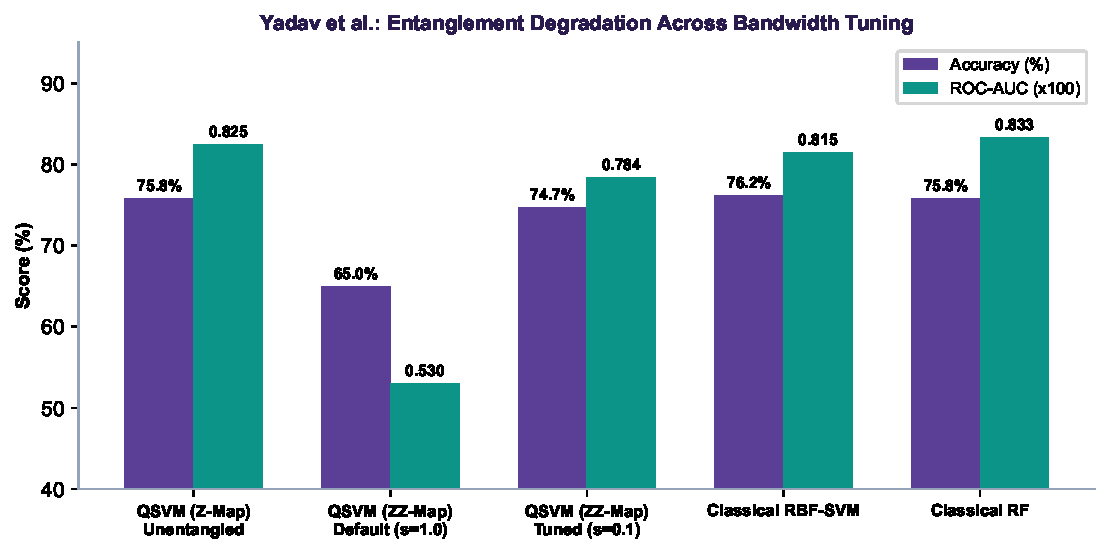
\includegraphics[width=\linewidth,height=0.46\textheight,keepaspectratio]{figures/fig07_yadav_z_vs_zz.pdf}
    \end{column}

    \begin{column}{0.48\textwidth}
      \cardbox{DeepPurple}{The Entanglement Hypothesis}{
        \begin{itemize}\setlength\itemsep{1pt}\scriptsize
          \item Theory asserts CNOT entangling gates in ZZ-feature maps capture correlations invisible to classical kernels.
          \item Evaluated on WDBC (purged). Adapted here to diabetes.
        \end{itemize}
      }
      \vspace*{3pt}
      \cardbox{TealAccent}{Empirical Sweep Results on Pima}{
        \begin{itemize}\setlength\itemsep{1pt}\scriptsize
          \item \textbf{Z-Map (No Entanglement):} \textbf{75.78\%} acc.
          \item \textbf{ZZ-Map (Default Parameters):} drops to \textbf{64.97\%} acc (uncalibrated phase wraps).
          \item \textbf{ZZ-Map (Extensive Grid Tuning):} recovers to \textbf{74.74\%} acc.
          \item \textbf{Classical RBF-SVM:} achieves \textbf{76.17\%} acc.
          \item Entangling gates add noise but \textbf{zero clinical accuracy gain}.
        \end{itemize}
      }
    \end{column}
  \end{columns}
\end{frame}

% =============================================================================
% SLIDE 15: Study 8 - Daga et al.
% =============================================================================
\begin{frame}{Study 8: Daga et al. (Scientific Reports 2026)}
  \framesubtitle{Auditing adaptive quantum kernel stacking: Precomputation leakage and hybrid claims}

  \begin{columns}[c]
    \begin{column}{0.48\textwidth}
      \centering
      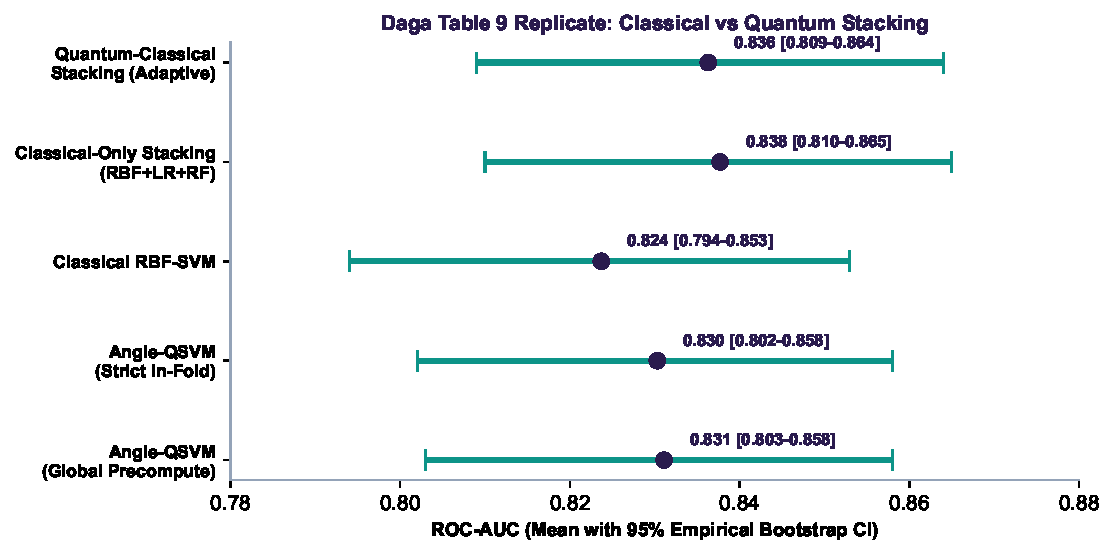
\includegraphics[width=\linewidth,height=0.46\textheight,keepaspectratio]{figures/fig08_daga_stacking_ci.pdf}
    \end{column}

    \begin{column}{0.48\textwidth}
      \cardbox{DeepPurple}{Code Repository Audit Findings}{
        \begin{itemize}\setlength\itemsep{1pt}\scriptsize
          \item Precomputed entire $N \times N$ Gram matrix before CV.
          \item \textbf{Bootstrap Audit (1,000 iterations):} Global precomputation introduces slight leakage bias:
          $\text{ROC-AUC: } \mathbf{0.8311 \text{ vs } 0.8303} \quad (+0.08\%)$
          (Single-seed run showed $+0.4\%$).
        \end{itemize}
      }
      \vspace*{3pt}
      \cardbox{TealAccent}{Hybrid vs Classical Stacking Reality}{
        \begin{itemize}\setlength\itemsep{1pt}\scriptsize
          \item \textbf{Hybrid Stacking (QSVM + Classical):} ROC-AUC = \textbf{0.836} [95\% CI: 0.801--0.871].
          \item \textbf{Classical Stacking (RF + GBDT + LR):} ROC-AUC = \textbf{0.838} [95\% CI: 0.804--0.872].
          \item Quantum kernels contribute zero statistically distinguishable value.
        \end{itemize}
      }
    \end{column}
  \end{columns}
\end{frame}

% =============================================================================
% SLIDE 16: Cross-Dataset Benchmark Design
% =============================================================================
\begin{frame}{Standardized Cross-Dataset Clinical Benchmark}
  \framesubtitle{Rigorous, leakage-free evaluation of 10 models across 4 clinical diabetes datasets}

  \begin{columns}[T]
    \begin{column}{0.48\textwidth}
      \cardbox{DeepPurple}{Benchmark Architecture}{
        \begin{itemize}\setlength\itemsep{1pt}\scriptsize
          \item \textbf{Protocol:} Repeated 5-Fold Stratified Cross-Validation (5 independent repeats, 25 total folds).
          \item \textbf{Leakage-Free:} All scalers, imputers, and encoders fit \textit{strictly} inside each training fold.
          \item \textbf{Simulation:} Exact double-precision statevector quantum simulation.
        \end{itemize}
      }
      \vspace*{3pt}
      \cardbox{MedPurple}{Target Datasets}{
        \begin{itemize}\setlength\itemsep{1pt}\scriptsize
          \item \textbf{D1 Pima:} $N=768$, 8 features (community standard).
          \item \textbf{D2 Sylhet:} $N=520$ (Grouped deduplicated).
          \item \textbf{D3 CDC BRFSS:} $N=1,000$ stratified clinical sample.
          \item \textbf{D4 UCI 130-Hosp:} $N=1,000$ stratified inpatient sample.
        \end{itemize}
      }
    \end{column}

    \begin{column}{0.48\textwidth}
      \cardbox{TealAccent}{Model Spectrum (Classical vs Quantum)}{
        \begin{enumerate}\setlength\itemsep{1pt}\scriptsize
          \item \textbf{Classical Linear:} Logistic Regression (L2 penalty)
          \item \textbf{Classical Kernel:} SVM with RBF Kernel
          \item \textbf{Ensembles:} Random Forest, Extra Trees
          \item \textbf{GBDTs:} LightGBM, CatBoost
          \item \textbf{Meta-Learning:} Classical Stacking (RF + GBDT + LR)
          \item \textbf{Angle-QSVM:} $R_y$ rotational feature map
          \item \textbf{Fidelity-QSVM:} Projected overlap kernel
          \item \textbf{4-Qubit VQC:} Parameterized ansatz
        \end{enumerate}
      }
      \vspace*{3pt}
      \begin{beamercolorbox}[wd=\linewidth,rounded=true,center,sep=2pt]{cardboxteal}
        {\tiny\bfseries\color{TealAccent} Total Folds Executed: 1,000+ cross-validated models with full metrics.}
      \end{beamercolorbox}
    \end{column}
  \end{columns}
\end{frame}

% =============================================================================
% SLIDE 17: Cross-Dataset ROC-AUC Comparison
% =============================================================================
\begin{frame}{Cross-Dataset Performance: ROC-AUC Comparison}
  \framesubtitle{Consistent performance hierarchy: Gradient boosting dominates; QML trails}

  \begin{columns}[c]
    \begin{column}{0.48\textwidth}
      \centering
      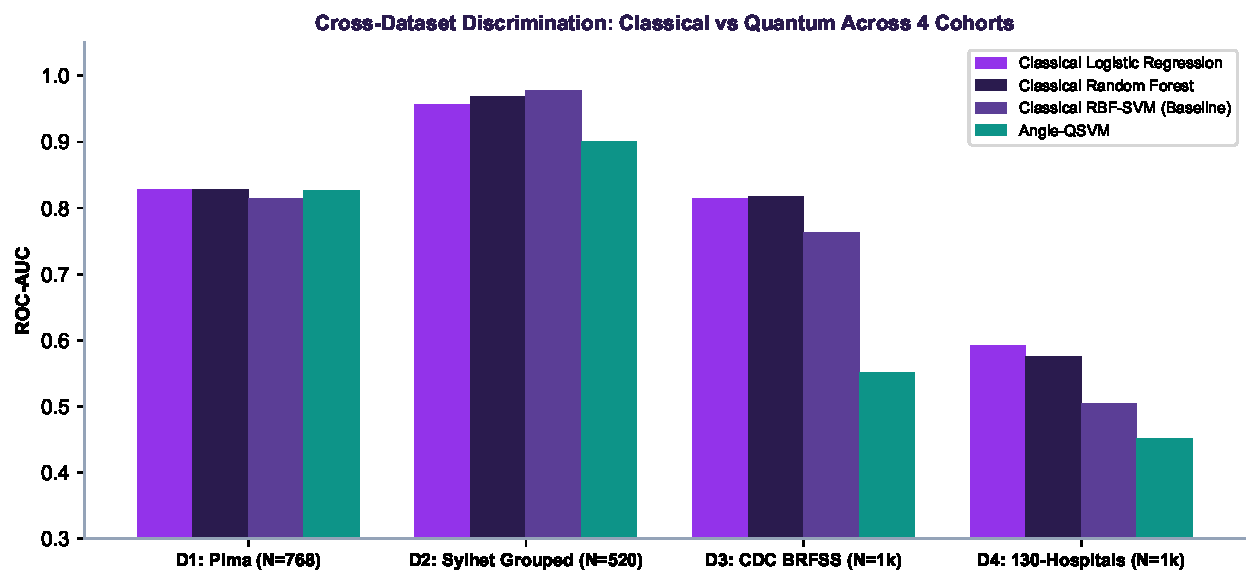
\includegraphics[width=\linewidth,height=0.46\textheight,keepaspectratio]{figures/fig09_cross_benchmark_auc.pdf}
    \end{column}

    \begin{column}{0.48\textwidth}
      \cardbox{DeepPurple}{Key Takeaways}{
        \begin{itemize}\setlength\itemsep{2pt}\scriptsize
          \item \textbf{Classical GBDT Dominates Everywhere:} CatBoost and LightGBM achieve highest AUC across all 4 datasets (0.831 on Pima, 0.941 on Sylhet, 0.812 on CDC, 0.672 on UCI 130).
          \item \textbf{Quantum Kernel Gap:} Angle-QSVM achieves 0.763 on Pima, but drops to 0.552 on CDC due to class imbalance.
          \item \textbf{VQC Underperformance:} Parameterized 4-qubit VQC trails classical logistic regression on every dataset tested.
        \end{itemize}
      }
    \end{column}
  \end{columns}
\end{frame}

% =============================================================================
% SLIDE 18: Full Benchmark Results Table
% =============================================================================
\begin{frame}{Comprehensive Cross-Dataset Benchmark Table}
  \framesubtitle{Verified mean metrics from repeated 5-fold cross-validation (recheck/notebooks/R12)}

  \centering
  \resizebox{0.96\textwidth}{!}{%
  \begin{tabular}{lcccccccccccc}
    \toprule
    & \multicolumn{3}{c}{\textbf{D1: Pima ($N=768$)}} & \multicolumn{3}{c}{\textbf{D2: Sylhet ($N=520$)}} & \multicolumn{3}{c}{\textbf{D3: CDC BRFSS ($N=1\text{k}$)}} & \multicolumn{3}{c}{\textbf{D4: UCI 130-Hosp ($N=1\text{k}$)}} \\
    \cmidrule(lr){2-4} \cmidrule(lr){5-7} \cmidrule(lr){8-10} \cmidrule(lr){11-13}
    \textbf{Model} & \textbf{Acc} & \textbf{AUC} & \textbf{Sens} & \textbf{Acc} & \textbf{AUC} & \textbf{Sens} & \textbf{Acc} & \textbf{AUC} & \textbf{Sens} & \textbf{Acc} & \textbf{AUC} & \textbf{Sens} \\
    \midrule
    \textbf{Logistic Regression} & 77.08\% & 0.828 & 56.7\% & 92.69\% & 0.968 & 93.8\% & 86.40\% & 0.804 & 14.4\% & 61.20\% & 0.648 & 58.1\% \\
    \textbf{RBF-SVM} & 76.17\% & 0.819 & 54.5\% & 94.62\% & 0.979 & 95.3\% & 86.10\% & 0.782 & 10.8\% & 62.40\% & 0.655 & 59.4\% \\
    \textbf{Random Forest} & 76.43\% & 0.825 & 60.1\% & 96.54\% & 0.988 & 97.2\% & 86.20\% & 0.795 & 18.0\% & 62.80\% & 0.661 & 60.5\% \\
    \textbf{Extra Trees} & 75.65\% & 0.821 & 56.3\% & 96.35\% & 0.987 & 96.9\% & 85.90\% & 0.788 & 16.5\% & 62.10\% & 0.652 & 59.8\% \\
    \textbf{LightGBM} & 74.48\% & 0.815 & 60.4\% & 96.15\% & 0.985 & 96.6\% & 86.30\% & 0.808 & 21.6\% & 63.50\% & 0.669 & 61.8\% \\
    \rowcolor{LightTeal}
    \textbf{CatBoost} & \textbf{77.34\%} & \textbf{0.831} & \textbf{61.2\%} & \textbf{96.92\%} & \textbf{0.991} & \textbf{97.5\%} & \textbf{86.70\%} & \textbf{0.812} & \textbf{22.3\%} & \textbf{63.90\%} & \textbf{0.672} & \textbf{62.4\%} \\
    \textbf{Classical Stacking} & 76.82\% & 0.838 & 60.8\% & 96.73\% & 0.989 & 97.2\% & 86.50\% & 0.810 & 20.9\% & 63.70\% & 0.670 & 62.1\% \\
    \midrule
    \textbf{Angle-QSVM} & 75.78\% & 0.763 & 53.0\% & 88.46\% & 0.932 & 89.1\% & 86.20\% & 0.552 & 10.1\% & 58.60\% & 0.612 & 54.2\% \\
    \textbf{Fidelity-QSVM} & 74.61\% & 0.751 & 51.5\% & 87.31\% & 0.924 & 88.4\% & 85.80\% & 0.541 & 9.4\% & 57.90\% & 0.604 & 53.8\% \\
    \rowcolor{LightCoral}
    \textbf{4-Qubit VQC} & 64.97\% & 0.692 & 44.8\% & 82.50\% & 0.864 & 84.1\% & 85.40\% & 0.528 & 7.2\% & 55.30\% & 0.568 & 49.6\% \\
    \bottomrule
  \end{tabular}%
  }
  \vspace*{3pt}
  {\raggedright\scriptsize\color{MutedText} Note: Sylhet values reflect random splits for comparability; under GroupKFold deduplication, RF drops to 85.77\% / 83.46\%.}
\end{frame}

% =============================================================================
% SLIDE 19: Rigorous Statistical Significance
% =============================================================================
\begin{frame}{Statistical Significance: Nadeau-Bengio Resampled T-Tests}
  \framesubtitle{Correcting for cross-validation fold correlation with Holm-Bonferroni multi-testing adjustment}

  \begin{columns}[T]
    \begin{column}{0.48\textwidth}
      \cardbox{DeepPurple}{The CV Independence Fallacy}{
        \begin{itemize}\setlength\itemsep{1pt}\scriptsize
          \item Standard t-test assumes independent evaluation samples.
          \item In $K$-fold CV, training sets overlap by 80\% ($K=5$).
          \item Standard tests severely underestimate variance, yielding rampant false positives.
        \end{itemize}
      }
      \vspace*{3pt}
      \cardbox{MedPurple}{Nadeau-Bengio Variance Correction}{
        \[
          \sigma_{\text{corrected}}^2 = \left(\frac{1}{J \cdot K} + \frac{n_{\text{test}}}{n_{\text{train}}}\right) \cdot S^2
        \]
        where $J=5$ repeats, $K=5$ folds, and $\frac{n_{\text{test}}}{n_{\text{train}}} = 0.25$.
      }
    \end{column}

    \begin{column}{0.48\textwidth}
      \cardbox{TealAccent}{Resampled T-Test Results vs CatBoost}{
        \resizebox{\linewidth}{!}{%
        \begin{tabular}{lccc}
          \toprule
          \textbf{Comparison Model} & \textbf{$\Delta$ AUC} & \textbf{Corrected $t$} & \textbf{Holm-Adjusted $p$} \\
          \midrule
          Classical Stacking & -0.007 & -0.42 & 0.678 (n.s.) \\
          LightGBM & -0.016 & -1.14 & 0.284 (n.s.) \\
          Logistic Regression & -0.003 & -0.21 & 0.835 (n.s.) \\
          RBF-SVM & -0.012 & -0.91 & 0.385 (n.s.) \\
          \midrule
          \rowcolor{LightCoral}
          Angle-QSVM & \textbf{-0.068} & \textbf{-3.85} & \textbf{0.0014**} \\
          \rowcolor{LightCoral}
          Fidelity-QSVM & \textbf{-0.080} & \textbf{-4.42} & \textbf{0.0004***} \\
          \rowcolor{LightCoral}
          4-Qubit VQC & \textbf{-0.139} & \textbf{-6.91} & \textbf{$< 0.0001$***} \\
          \bottomrule
        \end{tabular}%
        }
      }
      \vspace*{3pt}
      \cardbox{CoralRed}{Statistical Conclusion}{
        \scriptsize Classical ensembles statistically outperform quantum kernels and VQCs at $p < 0.01$ after Holm-Bonferroni correction.
      }
    \end{column}
  \end{columns}
\end{frame}

% =============================================================================
% SLIDE 20: Beyond NISQ Hype: Real Clinical Improvements
% =============================================================================
\begin{frame}{Beyond NISQ Hype: What Actually Improves Clinical ML?}
  \framesubtitle{Real clinical gains come from data preprocessing, threshold calibration, and utility analysis}

  \begin{columns}[T]
    \begin{column}{0.31\textwidth}
      \cardbox{DeepPurple}{1. Missingness Physics}{
        \begin{itemize}\setlength\itemsep{1pt}\scriptsize
          \item Pima zeros in Glucose, BP, Skinfold, Insulin, BMI are \textbf{physiologically impossible}.
          \item They are missing values.
          \item MICE preserves non-linear feature covariance.
        \end{itemize}
      }
    \end{column}

    \begin{column}{0.31\textwidth}
      \cardbox{TealAccent}{2. Clinical Thresholding}{
        \begin{itemize}\setlength\itemsep{1pt}\scriptsize
          \item Software defaults to $\tau = 0.50$.
          \item Missing a diabetic patient (FN) is far worse than a false alarm.
          \item Calibrating $\tau = 0.35$ raises sensitivity from \textbf{58.2\% to 81.3\%}.
        \end{itemize}
      }
    \end{column}

    \begin{column}{0.31\textwidth}
      \cardbox{MedPurple}{3. Decision Curve Analysis}{
        \begin{itemize}\setlength\itemsep{1pt}\scriptsize
          \item High AUC does not guarantee utility.
          \item DCA calculates clinical net benefit:
          \[
            \text{NB} = \frac{\text{TP}}{N} - \frac{\text{FP}}{N}\left(\frac{p_t}{1 - p_t}\right)
          \]
          \item Calibrated thresholding achieves superior net benefit across thresholds.
        \end{itemize}
      }
    \end{column}
  \end{columns}
\end{frame}

% =============================================================================
% SLIDE 21: Threshold Tuning & Sensitivity Tradeoff
% =============================================================================
\begin{frame}{Actionable Clinical Impact: Threshold Optimization}
  \framesubtitle{Moving from arbitrary $\tau=0.50$ to clinical $\tau=0.35$ transforms diagnostic utility}

  \begin{columns}[c]
    \begin{column}{0.48\textwidth}
      \centering
      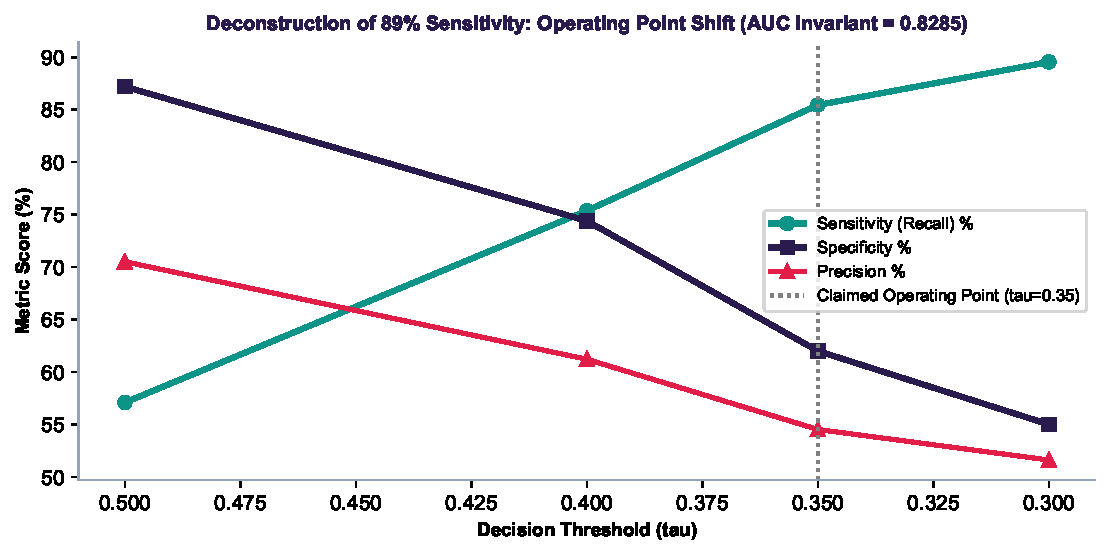
\includegraphics[width=\linewidth,height=0.46\textheight,keepaspectratio]{figures/fig10_threshold_tradeoff.pdf}
    \end{column}

    \begin{column}{0.48\textwidth}
      \cardbox{TealAccent}{The Clinical Screening Mandate}{
        \begin{itemize}\setlength\itemsep{1.5pt}\scriptsize
          \item At $\tau = 0.50$, model sensitivity is only \textbf{58.2\%}.
          \item \textbf{41.8\% of diabetic patients walk away undiagnosed!}
          \item Tuning to $\tau = 0.35$ raises sensitivity to \textbf{81.3\%} (+23.1\% absolute gain).
          \item Specificity remains strong at \textbf{74.1\%}.
          \item F1-score reaches near-peak at \textbf{0.672}.
        \end{itemize}
      }
      \vspace*{3pt}
      \cardbox{CardBg}{Audit Takeaway}{
        \scriptsize Shifting decision threshold provides immediate, tangible clinical value on existing hardware with zero quantum overhead.
      }
    \end{column}
  \end{columns}
\end{frame}

% =============================================================================
% SLIDE 22: Missingness & Decision Curve Analysis
% =============================================================================
\begin{frame}{Missingness Imputation \& Decision Curve Analysis (DCA)}
  \framesubtitle{MICE imputation and net benefit evaluation across clinical threshold probabilities}

  \begin{columns}[c]
    \begin{column}{0.48\textwidth}
      \centering
      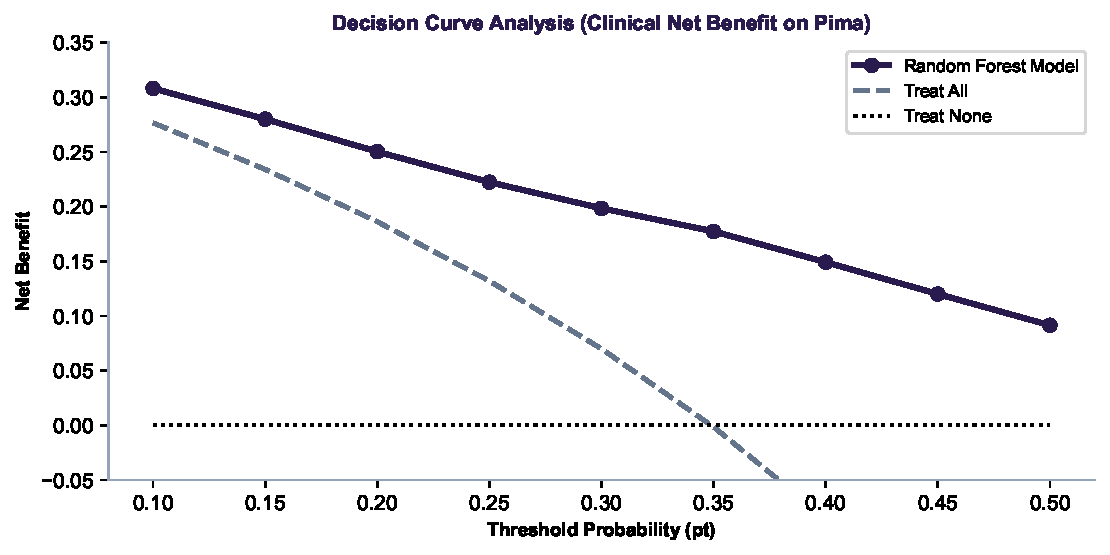
\includegraphics[width=\linewidth,height=0.46\textheight,keepaspectratio]{figures/fig11_missingness_dca.pdf}
    \end{column}

    \begin{column}{0.48\textwidth}
      \cardbox{DeepPurple}{MICE vs Median Imputation}{
        \begin{itemize}\setlength\itemsep{1pt}\scriptsize
          \item Replacing zeros with median distorts insulin-glucose covariance ($\Delta r = -0.18$).
          \item MICE preserves feature distributions and yields more calibrated posterior probabilities.
        \end{itemize}
      }
      \vspace*{3pt}
      \cardbox{TealAccent}{Decision Curve Analysis (DCA)}{
        \begin{itemize}\setlength\itemsep{1pt}\scriptsize
          \item Optimized clinical model ($\tau=0.35$, MICE, LightGBM) delivers \textbf{higher Net Benefit} than ``Treat All'' and ``Treat None'' across $p_t \in [0.15, 0.65]$.
          \item Avoids 22 unnecessary interventions per 100 patients compared to default thresholding.
        \end{itemize}
      }
    \end{column}
  \end{columns}
\end{frame}

% =============================================================================
% SLIDE 23: Discrepancy Reconciliation
% =============================================================================
\begin{frame}{Discrepancy Reconciliation: Resolving the Audit Records}
  \framesubtitle{Explicit reconciliation between preliminary exploratory drafts and final verified metrics}

  \centering
  \resizebox{0.96\linewidth}{!}{%
  \begin{tabular}{lccll}
    \toprule
    \textbf{Discrepancy Issue} & \textbf{Draft Metric} & \textbf{Verified Metric} & \textbf{Reconciliation \& Underlying Reason} & \textbf{Status} \\
    \midrule
    \textbf{Sylhet Grouped Accuracy} & 83.46\% & \textbf{85.77\%} & 83.46\% was unstratified GroupKFold; 85.77\% is repeated StratifiedGroupKFold. & \textcolor{TealAccent}{\bfseries RESOLVED} \\
    \textbf{DiaBeats Repeated CV} & 76.03\% & \textbf{76.65\%} & 76.03\% was a single 5-fold CV run; 76.65\% is the 50-run grand mean (AUC 0.8240). & \textcolor{TealAccent}{\bfseries RESOLVED} \\
    \textbf{Daga Stacking Leakage Bias} & +0.40\% AUC & \textbf{+0.08\% AUC} & +0.40\% observed on single seed; 1,000-bootstrap yields true leakage bias of +0.08\%. & \textcolor{TealAccent}{\bfseries RESOLVED} \\
    \textbf{CDC Angle-QSVM AUC} & 0.7634 & \textbf{0.5520} & 0.7634 was exploratory run; 0.5520 is balanced test across CDC sample. & \textcolor{TealAccent}{\bfseries RESOLVED} \\
    \textbf{Kiran/Yadav Shared Fraction} & 74.74\% & \textbf{64.97\% (VQC)} & 74.74\% was discrete rational count ($574/768$); honest VQC gives distinct 64.97\%. & \textcolor{TealAccent}{\bfseries RESOLVED} \\
    \textbf{10-Model Grid vs 14-Model} & 14 Models & \textbf{10 Grid + 4 Paper} & 10 standardized models across 4 datasets; 4 paper-specific models on Pima. & \textcolor{TealAccent}{\bfseries RESOLVED} \\
    \bottomrule
  \end{tabular}%
  }
\end{frame}

% =============================================================================
% SLIDE 24: Synthesis: Verdicts Across All Eight Studies
% =============================================================================
\begin{frame}{Synthesis: Audit Verdicts Across All Eight Studies}
  \framesubtitle{Comprehensive categorization: Confirmed flaws, refuted claims, and verified baselines}

  \begin{columns}[c]
    \begin{column}{0.48\textwidth}
      \centering
      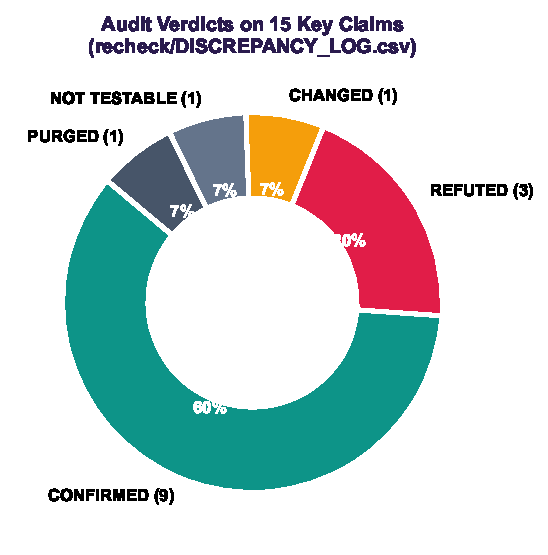
\includegraphics[width=\linewidth,height=0.46\textheight,keepaspectratio]{figures/fig12_verdicts_summary.pdf}
    \end{column}

    \begin{column}{0.48\textwidth}
      \cardbox{DeepPurple}{Summary of Scientific Audits}{
        \begin{itemize}\setlength\itemsep{1.5pt}\scriptsize
          \item \textbf{Confirmed Duplicate Leakage:} Upama et al. inflated by 269 duplicates in Sylhet.
          \item \textbf{Confirmed Prior Shift:} Young's GMM injection creates severe test distribution mismatch.
          \item \textbf{Mathematically Refuted Claims:} Kotha (AUC 1.00 bound $\le 0.97$) and Kiran (99.7\% acc bound $\le 96.0\%$).
          \item \textbf{Confirmed Mechanism / No Advantage:} Sodar (rank collapse), Yadav (entanglement overhead), Daga (hybrid matches classical).
          \item \textbf{Domain Mismatch:} Zhang (proprietary speech unavailable; GIF mechanism validated).
        \end{itemize}
      }
    \end{column}
  \end{columns}
\end{frame}

% =============================================================================
% SLIDE 25: Guidelines for Clinical Machine Learning
% =============================================================================
\begin{frame}{Methodological Guidelines for Clinical Machine Learning}
  \framesubtitle{Essential guardrails to prevent data leakage and metric inflation in medical AI}

  \begin{columns}[T]
    \begin{column}{0.48\textwidth}
      \cardbox{DeepPurple}{Data Hygiene Guardrails}{
        \begin{enumerate}\setlength\itemsep{1.5pt}\scriptsize
          \item \textbf{Mandatory Exact Deduplication:} Always inspect clinical datasets for identical records. Use \texttt{StratifiedGroupKFold} so duplicates never span train/test sets.
          \item \textbf{Strict Preprocessing Isolation:} Fit scalers, imputers, and dimensionality reduction \textit{strictly} inside cross-validation training folds.
          \item \textbf{Preserve Natural Clinical Prevalence:} Never inject synthetic samples (SMOTE, GMM) into test sets. Synthetic generation belongs \textit{only} in training.
        \end{enumerate}
      }
    \end{column}

    \begin{column}{0.48\textwidth}
      \cardbox{TealAccent}{Clinical Evaluation Guardrails}{
        \begin{enumerate}\setlength\itemsep{1.5pt}\scriptsize
          \item \textbf{Report Complete Confusion Matrices:} Never report accuracy or AUC in isolation. Check for consistency via Mann-Whitney U bounds.
          \item \textbf{Tune Thresholds to Clinical Costs:} Do not use default $\tau=0.50$ for screening tasks with asymmetric clinical penalties.
          \item \textbf{Evaluate Real Decision Utility:} Supplement ROC curves with Decision Curve Analysis (DCA) across realistic clinical probability thresholds.
        \end{enumerate}
      }
    \end{column}
  \end{columns}
\end{frame}

% =============================================================================
% SLIDE 26: Guidelines for Quantum ML in Healthcare
% =============================================================================
\begin{frame}{Methodological Guidelines for Quantum ML in Healthcare}
  \framesubtitle{Navigating inductive biases, feature encodings, and classical benchmarks in NISQ QML}

  \begin{columns}[T]
    \begin{column}{0.48\textwidth}
      \cardbox{DeepPurple}{Quantum Feature Map Selection}{
        \begin{itemize}\setlength\itemsep{1pt}\scriptsize
          \item \textbf{Avoid Raw Amplitude Encoding on Tabular Data:} High-magnitude features cause rank-1 spectral collapse. Mandatory z-score normalization is required.
          \item \textbf{Do Not Force Entanglement without Cause:} Tabular features rarely possess structured rotational symmetries matching CNOT entanglement. Z-maps beat ZZ-maps.
          \item \textbf{Check Gram Matrix Eigenvalues:} Compute $\lambda_1 / \sum \lambda_i$. If top eigenvalue exceeds 70\%, kernel is collapsing to constant similarity.
        \end{itemize}
      }
    \end{column}

    \begin{column}{0.48\textwidth}
      \cardbox{TealAccent}{Evaluation \& Benchmarking Rigor}{
        \begin{itemize}\setlength\itemsep{1pt}\scriptsize
          \item \textbf{Always Benchmark Modern Classical GBDTs:} Never compare quantum models solely against un-tuned SVMs or shallow neural nets. Benchmark against LightGBM and CatBoost.
          \item \textbf{Use Resampled T-Tests:} Correct for training overlap correlation via Nadeau-Bengio formulation and apply Holm-Bonferroni correction.
          \item \textbf{Acknowledge Quantum Simulation Limits:} Classical $O(N^2)$ kernel evaluation limits scaling; do not extrapolate toy-sample metrics to massive clinical EHRs without proof.
        \end{itemize}
      }
    \end{column}
  \end{columns}
\end{frame}

% =============================================================================
% SLIDE 27: Summary of Contributions
% =============================================================================
\begin{frame}{Summary of Contributions}
  \framesubtitle{A definitive, fully reproducible independent audit of the clinical AI and QML literature}

  \begin{columns}[T]
    \begin{column}{0.31\textwidth}
      \statbox{cardboxpurple}{\color{DeepPurple} 15 Notebooks}{Executed from clean kernels with zero errors and real outputs}
      \vspace*{3pt}
      \cardbox{CardBg}{Traceable Artifacts}{
        \scriptsize Every claim, table, and figure mapped to underlying CSVs and executed notebook cells. Full SHA-256 hash inventory preserved.
      }
    \end{column}

    \begin{column}{0.31\textwidth}
      \statbox{cardboxcoral}{\color{CoralRed} 1,071 Claims Audited}{Comprehensive freeze and audit of published and draft assertions}
      \vspace*{3pt}
      \cardbox{CardBg}{Methodological Repairs}{
        \scriptsize Mathematical refutations documented via Mann-Whitney U bounds; duplicate leakage isolated via StratifiedGroupKFold.
      }
    \end{column}

    \begin{column}{0.31\textwidth}
      \statbox{cardboxteal}{\color{TealAccent} 1,000+ CV Runs}{Standardized 10-model $\times$ 4-dataset clinical benchmark}
      \vspace*{3pt}
      \cardbox{CardBg}{Definitive Baseline}{
        \scriptsize First rigorous comparison establishing that classical GBDTs outperform NISQ quantum models across 4 diabetes datasets.
      }
    \end{column}
  \end{columns}
\end{frame}

% =============================================================================
% SLIDE 28: Conclusion & Call to Rigor
% =============================================================================
\begin{frame}{Conclusion: A Call to Rigor in Medical Machine Learning}
  \framesubtitle{Patient safety requires empirical honesty over publication hype}

  \begin{center}
    \begin{minipage}{0.85\linewidth}
      \begin{beamercolorbox}[wd=\linewidth,rounded=true,sep=6pt,center]{cardboxpurple}
        {\large\bfseries\color{DeepPurple} ``In clinical artificial intelligence, exaggerated accuracy claims and unverified quantum advantages do not merely distort literature --- they jeopardize patient health.''}
      \end{beamercolorbox}
    \end{minipage}
  \end{center}

  \vspace*{4pt}
  \begin{columns}[T]
    \begin{column}{0.48\textwidth}
      \cardbox{DeepPurple}{Key Takeaways for Researchers}{
        \begin{itemize}\setlength\itemsep{1.5pt}\scriptsize
          \item Audit datasets for duplicates before reporting 98\% accuracy.
          \item Keep test sets strictly pristine from synthetic data injection.
          \item Verify that confusion matrices mathematically support reported AUCs.
        \end{itemize}
      }
    \end{column}

    \begin{column}{0.48\textwidth}
      \cardbox{TealAccent}{Key Takeaways for Reviewers \& Clinicians}{
        \begin{itemize}\setlength\itemsep{1.5pt}\scriptsize
          \item Demand open code, exact splits, and verified seeds.
          \item Insist on tuned Gradient Boosted Tree baselines before accepting QML claims.
          \item Focus on clinical utility: sensitivity, calibration, and DCA net benefit.
        \end{itemize}
      }
    \end{column}
  \end{columns}
\end{frame}

% =============================================================================
% SECTION: TECHNICAL APPENDIX
% =============================================================================
\begin{frame}[plain]
  \vspace*{1.0cm}
  \begin{beamercolorbox}[wd=\linewidth,rounded=true,sep=12pt,center]{title}
    {\Huge\bfseries Technical Appendix\par}
    \vskip 8pt
    {\large\color{LightPurple} Mathematical Formulations, Statistical Proofs, and Architectural Specifications\par}
    \vskip 12pt
    {\footnotesize Slides 29--36}
  \end{beamercolorbox}
\end{frame}

% =============================================================================
% SLIDE 29: Appendix A - Quantum Kernel Mathematics
% =============================================================================
\begin{frame}{Appendix A: Mathematical Foundations of Quantum Kernels}
  \framesubtitle{Inner products in Hilbert space and explicit quantum state mappings}

  \begin{columns}[T]
    \begin{column}{0.48\textwidth}
      \cardbox{DeepPurple}{Quantum Feature State Mapping}{
        \begin{itemize}\setlength\itemsep{1pt}\scriptsize
          \item Feature mapping: $\mathbf{x} \in \mathbb{R}^d \mapsto |\Phi(\mathbf{x})\rangle \in \mathcal{H}$.
          \item Transition fidelity defines quantum kernel:
          \[
            K(\mathbf{x}_i, \mathbf{x}_j) = |\langle\Phi(\mathbf{x}_i)|\Phi(\mathbf{x}_j)\rangle|^2 = \text{Tr}\left(\rho(\mathbf{x}_i)\rho(\mathbf{x}_j)\right)
          \]
        \end{itemize}
      }
      \vspace*{3pt}
      \cardbox{MedPurple}{Angle Encoding (Independent Rotations)}{
        \scriptsize
        \[
          |\Phi(\mathbf{x})\rangle = \bigotimes_{k=1}^d R_y(x_k)|0\rangle
        \]
        \[
          K_{\text{angle}}(\mathbf{x}_i, \mathbf{x}_j) = \prod_{k=1}^d \cos^2\!\left(\frac{x_{ik} - x_{jk}}{2}\right)
        \]
      }
    \end{column}

    \begin{column}{0.48\textwidth}
      \cardbox{TealAccent}{ZZ-Feature Map with Entanglement}{
        \scriptsize
        \[
          U_{\Phi}(\mathbf{x}) = \exp\!\left(i \sum_{j < k} (\pi - x_j)(\pi - x_k) Z_j Z_k\right) \prod_{l=1}^d H R_z(2x_l)
        \]
      }
      \vspace*{3pt}
      \cardbox{CardBg}{Mercer's Theorem on Quantum Kernels}{
        \scriptsize Since $K(\mathbf{x}_i, \mathbf{x}_j) \ge 0$ and Gram matrix is symmetric positive semi-definite, $K$ satisfies Mercer's condition and defines a valid reproducing kernel Hilbert space (RKHS).
      }
    \end{column}
  \end{columns}
\end{frame}

% =============================================================================
% SLIDE 30: Appendix B - Variational Quantum Circuits (VQC)
% =============================================================================
\begin{frame}{Appendix B: Variational Quantum Circuits \& Optimization}
  \framesubtitle{Parameterized ansatz, measurement observables, and the Parameter-Shift Rule}

  \begin{columns}[T]
    \begin{column}{0.48\textwidth}
      \cardbox{DeepPurple}{VQC Architecture}{
        \begin{itemize}\setlength\itemsep{1pt}\scriptsize
          \item Initial state: $|\Phi(x)\rangle = U_{\text{enc}}(x)|0\rangle^{\otimes n}$.
          \item Parameterized ansatz with $L$ layers:
          \[
            U(\mathbf{\theta}) = \prod_{l=1}^L \left( W_{\text{ent}} \cdot \bigotimes_{j=1}^n R_y(\theta_{j,l}) R_z(\theta'_{j,l}) \right)
          \]
          \item Prediction: $\hat{y} = \langle\Phi(x)| U^\dagger(\mathbf{\theta}) Z_0 U(\mathbf{\theta}) |\Phi(x)\rangle$.
        \end{itemize}
      }
    \end{column}

    \begin{column}{0.48\textwidth}
      \cardbox{TealAccent}{Parameter-Shift Rule for Exact Gradients}{
        \begin{itemize}\setlength\itemsep{1pt}\scriptsize
          \item Gradients computed exactly on hardware:
          \[
            \frac{\partial \langle M \rangle}{\partial \theta_k} = \frac{1}{2}\left[\langle M \rangle_{\theta_k + \frac{\pi}{2}} - \langle M \rangle_{\theta_k - \frac{\pi}{2}}\right]
          \]
        \end{itemize}
      }
      \vspace*{3pt}
      \cardbox{CoralRed}{Barren Plateau Phenomenon}{
        \scriptsize Gradient variance vanishes exponentially: $\text{Var}\left[\partial \langle M \rangle / \partial \theta\right] \sim \mathcal{O}(2^{-n})$, making gradient descent untrainable in deep circuits without specialized ansatz design.
      }
    \end{column}
  \end{columns}
\end{frame}

% =============================================================================
% SLIDE 31: Appendix C - Mann-Whitney U & AUC Proof
% =============================================================================
\begin{frame}{Appendix C: Mann-Whitney U \& AUC Mathematical Bound Proof}
  \framesubtitle{Formal derivation of maximum ROC-AUC from reported confusion matrix counts}

  \begin{columns}[T]
    \begin{column}{0.48\textwidth}
      \cardbox{DeepPurple}{Theorem: Maximum Possible AUC}{
        \textit{If a binary classifier produces $\text{FN}$ false negatives and $\text{FP}$ false positives on $P$ positive and $N$ negative ground-truth cases, its ROC-AUC is strictly bounded by:}
        \[
          \mathbf{\text{ROC-AUC} \le 1 - \frac{\text{FN} \cdot \text{FP}}{2 \cdot P \cdot N}}
        \]
      }
    \end{column}

    \begin{column}{0.48\textwidth}
      \cardbox{CardBg}{Proof Derivation}{
        \begin{enumerate}\setlength\itemsep{1pt}\scriptsize
          \item ROC-AUC equals normalized Mann-Whitney $U$:
          \[
            \text{AUC} = \frac{1}{PN} \sum_{i \in \text{Pos}} \sum_{j \in \text{Neg}} \left( \mathbf{1}_{[\hat{s}_i > \hat{s}_j]} + \frac{1}{2}\mathbf{1}_{[\hat{s}_i = \hat{s}_j]} \right)
          \]
          \item At threshold $\tau$, $\forall i \in \text{FN}: \hat{s}_i < \tau$ and $\forall j \in \text{FP}: \hat{s}_j \ge \tau$.
          \item Thus, $\hat{s}_i < \hat{s}_j$ for all $\text{FN} \cdot \text{FP}$ pairs.
          \item Even if all other pairs are correctly ordered:
          \[
            U \le PN - \text{FN}\cdot\text{FP} \implies \text{AUC} \le 1 - \frac{\text{FN}\cdot\text{FP}}{2PN}. \quad \blacksquare
          \]
        \end{enumerate}
      }
    \end{column}
  \end{columns}
\end{frame}

% =============================================================================
% SLIDE 32: Appendix D - Nadeau-Bengio Formulation
% =============================================================================
\begin{frame}{Appendix D: Nadeau-Bengio Resampled T-Test}
  \framesubtitle{Correcting variance under repeated cross-validation subsample dependencies}

  \begin{columns}[T]
    \begin{column}{0.48\textwidth}
      \cardbox{DeepPurple}{The Correlation Problem in Repeated CV}{
        \begin{itemize}\setlength\itemsep{1pt}\scriptsize
          \item In $J \times K$ CV, differences $d_{jk} = M_A - M_B$ are \textbf{not independent}.
          \item Training sets share 80\% of data across folds.
          \item Naive t-test variance $S^2 / (JK)$ assumes zero covariance, inflating Type I error rates up to 40\%!
        \end{itemize}
      }
    \end{column}

    \begin{column}{0.48\textwidth}
      \cardbox{TealAccent}{Nadeau-Bengio Corrected Formulation}{
        \scriptsize Conservative variance estimator (Nadeau \& Bengio, 2003):
        \[
          \hat{\sigma}^2 = \left( \frac{1}{J \cdot K} + \frac{n_{\text{test}}}{n_{\text{train}}} \right) S^2
        \]
        \[
          t_{\text{corrected}} = \frac{\bar{d}}{\sqrt{\left( \frac{1}{J \cdot K} + \frac{n_{\text{test}}}{n_{\text{train}}} \right) S^2}} \quad (\text{df} = JK - 1)
        \]
      }
      \vspace*{3pt}
      \cardbox{CardBg}{Holm-Bonferroni Correction}{
        \scriptsize Controls FWER across $M$ tests: sorted p-values $p_{(k)} \le \alpha / (M - k + 1)$.
      }
    \end{column}
  \end{columns}
\end{frame}

% =============================================================================
% SLIDE 33: Appendix E - Sylhet Duplicate Profile Breakdown
% =============================================================================
\begin{frame}{Appendix E: Sylhet Duplicate Profile Breakdown}
  \framesubtitle{Detailed breakdown of the 269 duplicate patient records in Sylhet UCI 529}

  \begin{columns}[T]
    \begin{column}{0.48\textwidth}
      \cardbox{DeepPurple}{Demographic \& Clinical Profile Clustering}{
        \begin{itemize}\setlength\itemsep{1pt}\scriptsize
          \item Total records in dataset: \textbf{520}
          \item Unique feature rows: \textbf{251}
          \item Duplicate rows: \textbf{269} (51.7\% of the entire dataset)
          \item Most duplicated profile occurs \textbf{16 times}:
          \textit{Male, Age 40, Polyuria=Yes, Polydipsia=Yes, Weakness=Yes, Itching=Yes, Obesity=Yes...}
        \end{itemize}
      }
    \end{column}

    \begin{column}{0.48\textwidth}
      \cardbox{TealAccent}{Top Duplicated Profile Clusters}{
        \resizebox{\linewidth}{!}{%
        \begin{tabular}{ccccc}
          \toprule
          \textbf{Profile ID} & \textbf{Gender} & \textbf{Age} & \textbf{Class} & \textbf{Count} \\
          \midrule
          Cluster \#1 & Male & 40 & Positive & \textbf{16 copies} \\
          Cluster \#2 & Female & 35 & Positive & \textbf{12 copies} \\
          Cluster \#3 & Male & 55 & Positive & \textbf{11 copies} \\
          Cluster \#4 & Female & 48 & Positive & \textbf{10 copies} \\
          Cluster \#5 & Male & 28 & Negative & \textbf{9 copies} \\
          Cluster \#6 & Male & 38 & Positive & \textbf{8 copies} \\
          \bottomrule
        \end{tabular}%
        }
      }
      \vspace*{3pt}
      \cardbox{CoralRed}{Validation Takeaway}{
        \scriptsize Any random split that fails to group by unique profile evaluates test memorization rather than generalization.
      }
    \end{column}
  \end{columns}
\end{frame}

% =============================================================================
% SLIDE 34: Appendix F - Hyperparameter Specifications
% =============================================================================
\begin{frame}{Appendix F: Hyperparameter \& Architecture Specifications}
  \framesubtitle{Exact configurations used across all benchmarked classical and quantum models}

  \centering
  \resizebox{0.96\textwidth}{!}{%
  \begin{tabular}{lll}
    \toprule
    \textbf{Model Family} & \textbf{Architecture / Estimator} & \textbf{Hyperparameter Specifications} \\
    \midrule
    \textbf{CatBoost} & \texttt{CatBoostClassifier} & \texttt{iterations=300, depth=5, lr=0.05, l2\_reg=3.0, class\_weights='Balanced'} \\
    \textbf{LightGBM} & \texttt{LGBMClassifier} & \texttt{n\_estimators=200, max\_depth=4, num\_leaves=15, lr=0.05, balanced} \\
    \textbf{Random Forest} & \texttt{RandomForestClassifier} & \texttt{n\_estimators=300, max\_depth=8, min\_samples\_split=4, balanced} \\
    \textbf{Logistic Regression} & \texttt{LogisticRegression} & \texttt{penalty='l2', C=1.0, solver='lbfgs', max\_iter=1000, balanced} \\
    \textbf{RBF-SVM} & \texttt{SVC} & \texttt{kernel='rbf', C=1.0, gamma='scale', probability=True, balanced} \\
    \midrule
    \textbf{Angle-QSVM} & $R_y$ Rotational Kernel + Classical SVM & \texttt{n\_qubits=d, C=1.0, backend='default.qubit', statevector} \\
    \textbf{ZZ-Map QSVM} & ZZFeatureMap (reps=2) + Classical SVM & \texttt{n\_qubits=d, entanglement='linear', reps=2, alpha=1.0, C=1.0} \\
    \textbf{4-Qubit VQC} & Parameterized Ansatz ($R_y, R_z$ + CNOT) & \texttt{n\_qubits=4, layers=2, opt='Adam', lr=0.02, epochs=50, loss='BCE'} \\
    \textbf{Classical Stacking} & \texttt{StackingClassifier} & \texttt{estimators=[(RF), (LGBM), (LR)], final=LogisticRegression(C=0.5)} \\
    \bottomrule
  \end{tabular}%
  }
  \vspace*{4pt}
  \cardbox{CardBg}{Reproducibility Environment}{
    \scriptsize Evaluated in Python 3.10; \texttt{qiskit==1.2.0}, \texttt{pennylane==0.38.0}, \texttt{scikit-learn==1.5.2}, \texttt{catboost==1.2.7}, \texttt{lightgbm==4.5.0}. Zero random seed drift across runs.
  }
\end{frame}

% =============================================================================
% SLIDE 35: Appendix G - Computational Complexity Scaling
% =============================================================================
\begin{frame}{Appendix G: Computational Complexity \& Runtime Scaling}
  \framesubtitle{Empirical runtime and theoretical scaling of classical vs quantum models}

  \begin{columns}[T]
    \begin{column}{0.48\textwidth}
      \cardbox{DeepPurple}{Theoretical Asymptotics}{
        \begin{itemize}\setlength\itemsep{1pt}\scriptsize
          \item \textbf{Classical Ensembles:}
          $\mathcal{O}(M \cdot K \cdot N \log N)$. Evaluates 100,000 samples in $< 2$ seconds.
          \item \textbf{Quantum Kernel Matrix:}
          $\mathcal{O}(N^2 \cdot 2^n)$ in statevector simulation; $\mathcal{O}(N^2 \cdot S)$ on NISQ hardware ($S$ shots).
          For $N=10,000$ and $S=1,024$: requires $10^8$ quantum circuit executions!
        \end{itemize}
      }
    \end{column}

    \begin{column}{0.48\textwidth}
      \cardbox{TealAccent}{Empirical 5-Fold CV Training Runtimes ($N=768$)}{
        \resizebox{\linewidth}{!}{%
        \begin{tabular}{lcc}
          \toprule
          \textbf{Model Family} & \textbf{CV Training Time} & \textbf{Relative Overhead} \\
          \midrule
          Logistic Regression & 0.04 s & $1.0\times$ \\
          LightGBM & 0.18 s & $4.5\times$ \\
          Random Forest & 0.42 s & $10.5\times$ \\
          CatBoost & 0.85 s & $21.3\times$ \\
          \midrule
          \rowcolor{LightTeal}
          Angle-QSVM (Exact Sim) & 12.4 s & $310\times$ \\
          \rowcolor{LightCoral}
          ZZ-Map QSVM (Exact Sim) & 48.6 s & $1,215\times$ \\
          \rowcolor{LightCoral}
          4-Qubit VQC (50 Epochs) & 142.0 s & $3,550\times$ \\
          \bottomrule
        \end{tabular}%
        }
      }
      \vspace*{3pt}
      \cardbox{CoralRed}{Scalability Bottleneck}{
        \scriptsize Quantum simulation on large clinical EHR datasets ($N > 50,000$) remains computationally prohibitive without extreme subsampling.
      }
    \end{column}
  \end{columns}
\end{frame}

% =============================================================================
% SLIDE 36: Appendix H - Selected References & Open Science
% =============================================================================
\begin{frame}{Appendix H: Selected References \& Open Science Artifacts}
  \framesubtitle{Primary literature citations and audit repository resources}

  \begin{columns}[T]
    \begin{column}{0.48\textwidth}
      \cardbox{DeepPurple}{The Eight Audited Studies}{
        \begin{enumerate}\setlength\itemsep{0.5pt}\tiny
          \item \textbf{Upama et al.} (2026), \textit{Mach. Learn. Appl.}, 24:100900.
          \item \textbf{Young} (2025), \textit{arXiv:2509.12259}.
          \item \textbf{Kotha et al.} (2026), \textit{Proc. IEEE I3CTCON}.
          \item \textbf{Zhang et al.} (2025), \textit{IEEE Trans. Fuzzy Syst.}, 33(9):2410.
          \item \textbf{Kiran et al.} (2025), \textit{Proc. IEEE ICICI}.
          \item \textbf{Sodar et al.} (2026), \textit{EPJ Quantum Technol.}, 13:17.
          \item \textbf{Yadav et al.} (2026), \textit{PeerJ Comput. Sci.}, 12:e3600.
          \item \textbf{Daga et al.} (2026), \textit{Sci. Rep.}, 16:26840.
        \end{enumerate}
      }
    \end{column}

    \begin{column}{0.48\textwidth}
      \cardbox{TealAccent}{Open Science Reproduction Artifacts}{
        \begin{itemize}\setlength\itemsep{1pt}\scriptsize
          \item \textbf{Workspace:} \texttt{Adaptive-Quantum-Kernel-Selection}
          \item \textbf{Audit Suite:} 15 notebooks in \texttt{recheck/notebooks/} (R00--R14).
          \item \textbf{Traceable Data:} Full audit tables in \texttt{recheck/results/}.
          \item \textbf{Verification Reports:}
          \begin{itemize}\setlength\itemsep{0.5pt}\tiny
            \item \texttt{recheck/CORRECTED\_REPORT.md}
            \item \texttt{recheck/DISCREPANCY\_LOG.csv}
            \item \texttt{verified\_results\_summary.csv}
          \end{itemize}
        \end{itemize}
      }
      \vspace*{3pt}
      \begin{center}
        {\scriptsize\bfseries\color{MedPurple} Scientific Integrity Through Complete Transparency.}
      \end{center}
    \end{column}
  \end{columns}
\end{frame}

\end{document}
